\chapter{Zestawienie zagadnień wykorzystanych w pracy}
\label{cha:Zestawienie zagadnień wykorzystanych w pracy}

\section{Mechaniczne układy napędowe}
\subsection{Przekładnie mechaniczne}
Układ napędowy to zestaw urządzeń wykorzystywany do napędzania, w skład którego wchodzi źrodło energii, układy pośredniczące w przekazywaniu energii oraz odbiornik energi. Mianem napędu zazwyczaj określa się urządzenia pośredniczące. Najczęściej wykorzystywanymi źródłami enrgii są silniki a odbirniki energii, których zadaniem jest realizowanie odpowiednich ruchów roboczych, przyjmują różne formy zależne od aplikacji.

Układ mechaniczny wykorzystany do przeniesienia ruchu obrotowego z elementu czynnego na element bierny nazywany jest przekładnią mechaniczną. Oprócz transmisji energii, przekładnie umożliwają również zmianę parametrów ruchu - momentu obrotowego oraz prędkości obrotowej. Przekładnie mechaniczne dzieli się na trzy grupy: cięgnowe, cierne i zębate. Przekładnie cięgnowe, które zostały opisane ze wzgędu na zastosowanie w rowerowych układach napędowych, składają się z conajmniej dwóch kół zębatych, rozsuniętych względem siebie, oraz cięgna opasającego. Ze względu na rodzaj zastosowanego cięgna, wyróżnia się przekładnie pasowe oraz łańcuchowe. Przenoszenie siły z cięgna na koło zębate jest możliwe dzięki zastosowaniu odpowiednich połączeń - połączenia cierne, kształtowe lub stałe przymocowanie cięgna do koła zębatego.

\textcolor{red}{@TODO wrzucić schemat przekładni, dodać jakiś przypis doprzełkadni}

Wielkością charakteryzującą przekładnie jest przełożenie. Wyróżnia się przełożenie geometryczne, kinematyczne oraz dynamiczne. Przełożenie kinematyczne to stosunek prędkości kątowej koła czynnego do prędkości kątowej koła biernego:
\textcolor{red}{@TODO wzorek i=w1/w2}

Przełożenie dynamiczne określa stosunek momentu obrotowego na kole biernym do momentu obrotowego koła czynnego.  

\textcolor{red}{@TODO wzorek i=M2/M1}

Przełożenie przekładni jest parametrem bezwymiarwoym. Ze względu na wartość przełożenia przekładni wyróznia się:
\begin{itemize}
\item
Przekładnie przyspieszające lub tzw. multiplikatory. Przekładnie tego typu zwiększają prędkość kątową koła biernego względem prędkości kątowej koła czynnego przy jednoczesnym zmniejszeniu momentu obrotowego koła biernego względem momentu obrotowego koła czynnego. Przełożenie takiej przekładni jest liczbą z zakresu od 0 do 1.
\item
Przekładnie redukujące lub tzw. reduktory. Przekładnie tego typu działają w sposób odwrotny do przekładni przyspieszających - zmniejszają prędkość kątową koła biernego względem prędkości kątowej koła czynnego oraz zwiększają moment obrotowy koła biernego wzlgędem momentu obrotowego koła czynnego. Przełożenei przekładni redukującej jest zawsze większe od 1.
\end{itemize} 


	  
\subsection{Układ napędowy w rowerze}
W przypadku konwencjonalnego układu napędowego stosowanego w rowerach źródłem energii jest rowerzysta. Siła przyłożona do ramienia korby generuje moment obrotowy, który przenoszony jest, przy pomocy mechanizmu korbowego i łańcucha, na koło zębate na stałe przymocowoane do piasty tylnego koła. Moment obrotowy koła napędzającego powoduje powstanie sił obwodowych, składających się na siłę napędową, która wprawia rower w ruch postępowy.

\section{Metody pomiarowe wielkości fizycznych}
\subsection{Pomiar prędkości kątowej oraz prędkości liniowej}

Możliwość pomiaru prędkości kątowej jest kluczowa ze względu na wykonanie trybu automatycznej zmiany przełożeń. Na podstawie aktualnej prędkości kątowej tylnego koła wyznaczona zostanie chwilowa prędkość liniowa. Pomiar prędkości kątowej mechanizmu korbowego umożliwi wyznaczenie aktulane wartości kadencji.

Prędkość kątowa jest wielkością wektorową, jednak w rozważaniach dotyczących pracy brana pod uwagę jest jedynie chwilowa wartość prędkości kątowej. Ta zdefiniowana jest jako zmiana drogi kątowej w czasie:
\begin{equation}
\omega = \frac{d\varphi}{dt}
\end{equation}
\begin{eqwhere}[2cm]
	\item[$\varphi$] droga kątowa
	\item[$t$] czas
\end{eqwhere}
Wyznaczenie chwilowej wartości prędkości kątowej wykonane zostało w oparciu o czujniki zbliżeniowy załączany magnetycznie, który został na stałe przymocowany do ramy roweru, w niewielkiej odległości od tylnego koła. Zasada działania takiego czujnika jest analogiczna do działania zwykłego przycisku monostabilnego. Obwód w czujniku jest domyślnie rozwarty. Zwarcie następuje w momencie zbliżenia magnesu do czujnika. Magnes przyczepiony został do szprychy roweru. Taki sam sposób pomiaru prędkości można znaleźć w komercyjnych licznikach rowerowych oferowanych na rynku. Autor zdecydował się na zastosowanie dwóch magnesów w celu zwiększenia dokładności pomiaru. Dysponując pomiarem czasu pomiędzy kolejnymi zwarciami czujnika magnetycznego, które, ze względu na zastosowanie dwóch magnesów, następują w wyniku obrotu koła o kąt $\pi$ , można wyznaczyć chwilową wartość prędkości kątowej: 
\begin{equation}
\omega = \frac{\pi}{T}
\end{equation}
\begin{eqwhere}[2cm]
	\item[$T$] czas od ostatniego zwarcia czujnika magnetycznego
\end{eqwhere}
Prędkość kątowa mechanizmu korbowego została wyznaczona w sposób analogiczny. Zbliżeniowy czujnik magnetyczny, który został na stałe przymocowany do ramy roweru, w bliskiej odległości mechanizmu korbowego, jest zwierany w każdym cyklu dzięki zastosowaniu magnesu, który został przyklejony do ramienia mechanizmu korbowego. Ze względu na zastosowanie jednego magnesu, przyrost drogi kątowej jest dwa razy większy, niż w przypadku pomiaru prędkości kątowej koła roweru i jego wartość wynosi 2$\pi$.

Wartość prędkości liniowej to stosunek przebytej drogi do czasu:
\begin{equation}
v = \frac{s}{t}
\end{equation}
\begin{eqwhere}[2cm]
	\item[$s$] droga liniowa
	\item[$v$] prędkość liniowa
\end{eqwhere}
 Związek pomiędzy drogą liniową a drogą kątową wyraża się wzorem:
\begin{equation}
\varphi = \frac{s}{r}
\end{equation}
\begin{eqwhere}[2cm]
	\item[$r$] promień okręgu
\end{eqwhere}
W układzie pomiarowym z dwoma magnesami, wartość drogi kątowej w momencie zwarcia czujnika magnetycznego wynosi $\pi$. Biorąc pod uwagę powyższe zależnosci, chwilowa wartość prędkości liniowej poruszającego się roweru może zostać wyznaczona z zależności:
 \begin{equation}
v = \frac{\pi R}{T}
\end{equation}
\begin{eqwhere}[2cm]
	\item[$R$] promień koła rowerowego
\end{eqwhere}
\subsection{Pomiar przyspieszeń}
Z drugiej zasady dynamiki Newtona wynika, iż przyspieszenie jest proporcjonalne do wypadkowej siły działającej na ciało. Znajomość chwilowej wartośći oraz zwrotu przyspieszenia jest drugą istotną informacją, która została wykorzystana przy projektowaniu sterownika trybu automatycznego, gdyż może dostarczyć wiedzy na temat dynamiki ruchu.

Pomiar przyspieszenia został zrealizowany w oparciu o zastosowanie akcelerometru wykonanego w technologii MEMS( z ang. {\em Micro Electro-Mechanical Systems}). Układy MEMS to urządzenia wykonane w miniaturowej skali, które integrują ze soba elementy mechaniczne oraz elektroniczne. Wykorzystywane głównie jako czujniki przetwarzające wielkości mechaniczne na wielkości elektryczne. Czujniki wykonane w technologii MEMS posiadają kilka znaczących zalet, które sprawiają, że spektrum zastosowań staje się coraz szersze. Są to m.in. niska cena, niewielkie rozmiary, niskie zużycie energii oraz prosta integracja z układami mikroprocesorowymi. Akcelerometry wykonane w tej technologii są powszechnie wykorzystywane w różnego rodzaju aplikacjach. Układy sterujące poduszkami powietrznymi, systemy alarmowe w samochodach czy tzw. asysten ruszania na wzniesieniu to tylko niektóre przykłady z branży motoryzacyjnej.

Akcelereometr to urządzenie pomiarowe, które umożliwia pomiar przyspieszenia dynamicznego ciała, na które działa niezerowa siła wypadkowa, oraz przyspieszenia statycznego ciała znajdującego się w ziemskim polu grawitacyjnym. Akcelerometry zazwyczaj działają na zasadzie przetworników pojemnościowych. Pomiar dokonywany jest dzięku zastosowaniu kondensatorów różnicowych, których ruchome okładki wychylane są z położenia równowagi pod wpływem działających sił bezwładności.

Akcelerometr wykonany w technologii MEMS zazwyczaj umożliwia pomiar przyspieszenia w trzech różnych kierunkach(\textcolor{red}{@TODO rysunek}). Akcelerometr został zamontowany w rowerze w taki sposób, aby kierunek osi \textit{X} był równoległy do podłoża. Dzięki temu wskazania akcelerometru wzdłuż osi X są proporcjonalne do siły wypadkowej działającej na rower.



\subsection{Pomiar kąta nachylenia}
Kąt nachylenia podłoża, po którym porusza się rower, to ostatnia z wielkości fizycznych brana pod uwagę przez algorytm automatycznej zmiany przełożeń. Wielkość ta wyznaczona zostanie pośrednio, poprzez analizę danych odczytywanych z akcelerometru. 

Przykład przedsatwiony na (\textcolor{red}{@TODO rysunek}) przedstawia rozkład rozkład przyspieszeń działających na caiło znajdujące się na równi pochyłej. Kąt nachylenia $\alpha$ można wyznaczyć z zależności:
\begin{equation}
\alpha=\arctan{\frac{a_{\parallel }}{a_{\bot }}}
\end{equation}
\begin{eqwhere}[2cm]
	\item[$\alpha$] kąt naychylenia podłoża
	\item[$a_{\parallel }$] kąt naychylenia podłoża
	\item[$a_{\bot }$] kąt naychylenia podłoża
\end{eqwhere}
\begin{center}
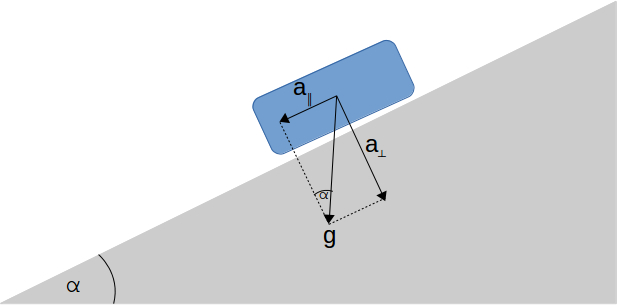
\includegraphics[scale=0.5]{dupa.jpg}
\end{center}
\section{Sterowanie}


\subsection{Zamknięty układ regulacji}
\subsection{Serwomechanizm}

\section{Kondycjonowanie sygnałów}


\subsection{Drganie styków}
\subsection{Filtr donlnoprzepustowy}